\section{Introduction}
\label{sec:intro}

%!TEX root = ../../main.tex
\begin{figure}[t]
    \centering 
    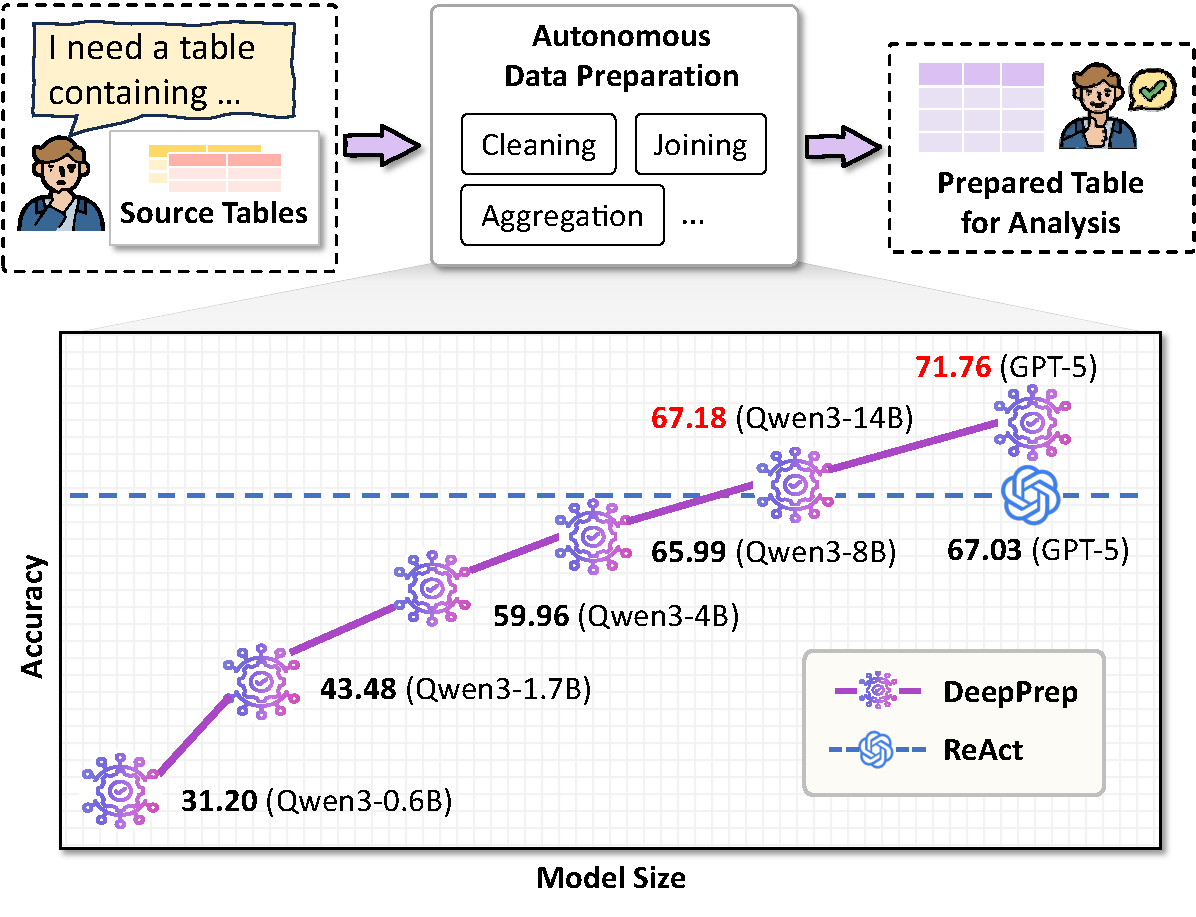
\includegraphics[width=0.85\columnwidth]{figures/fig/introduction_experiment.pdf}
    \vspace{-1em}
    \caption{Overview of Autonomous Data Preparation (Top) and Performance of \sys (Bottom).}
    \label{fig:introduction_experiment}
    \vspace{-1em}
\end{figure}
%!TEX root = ../../main.tex
\begin{figure*}[!t]
    \centering 
    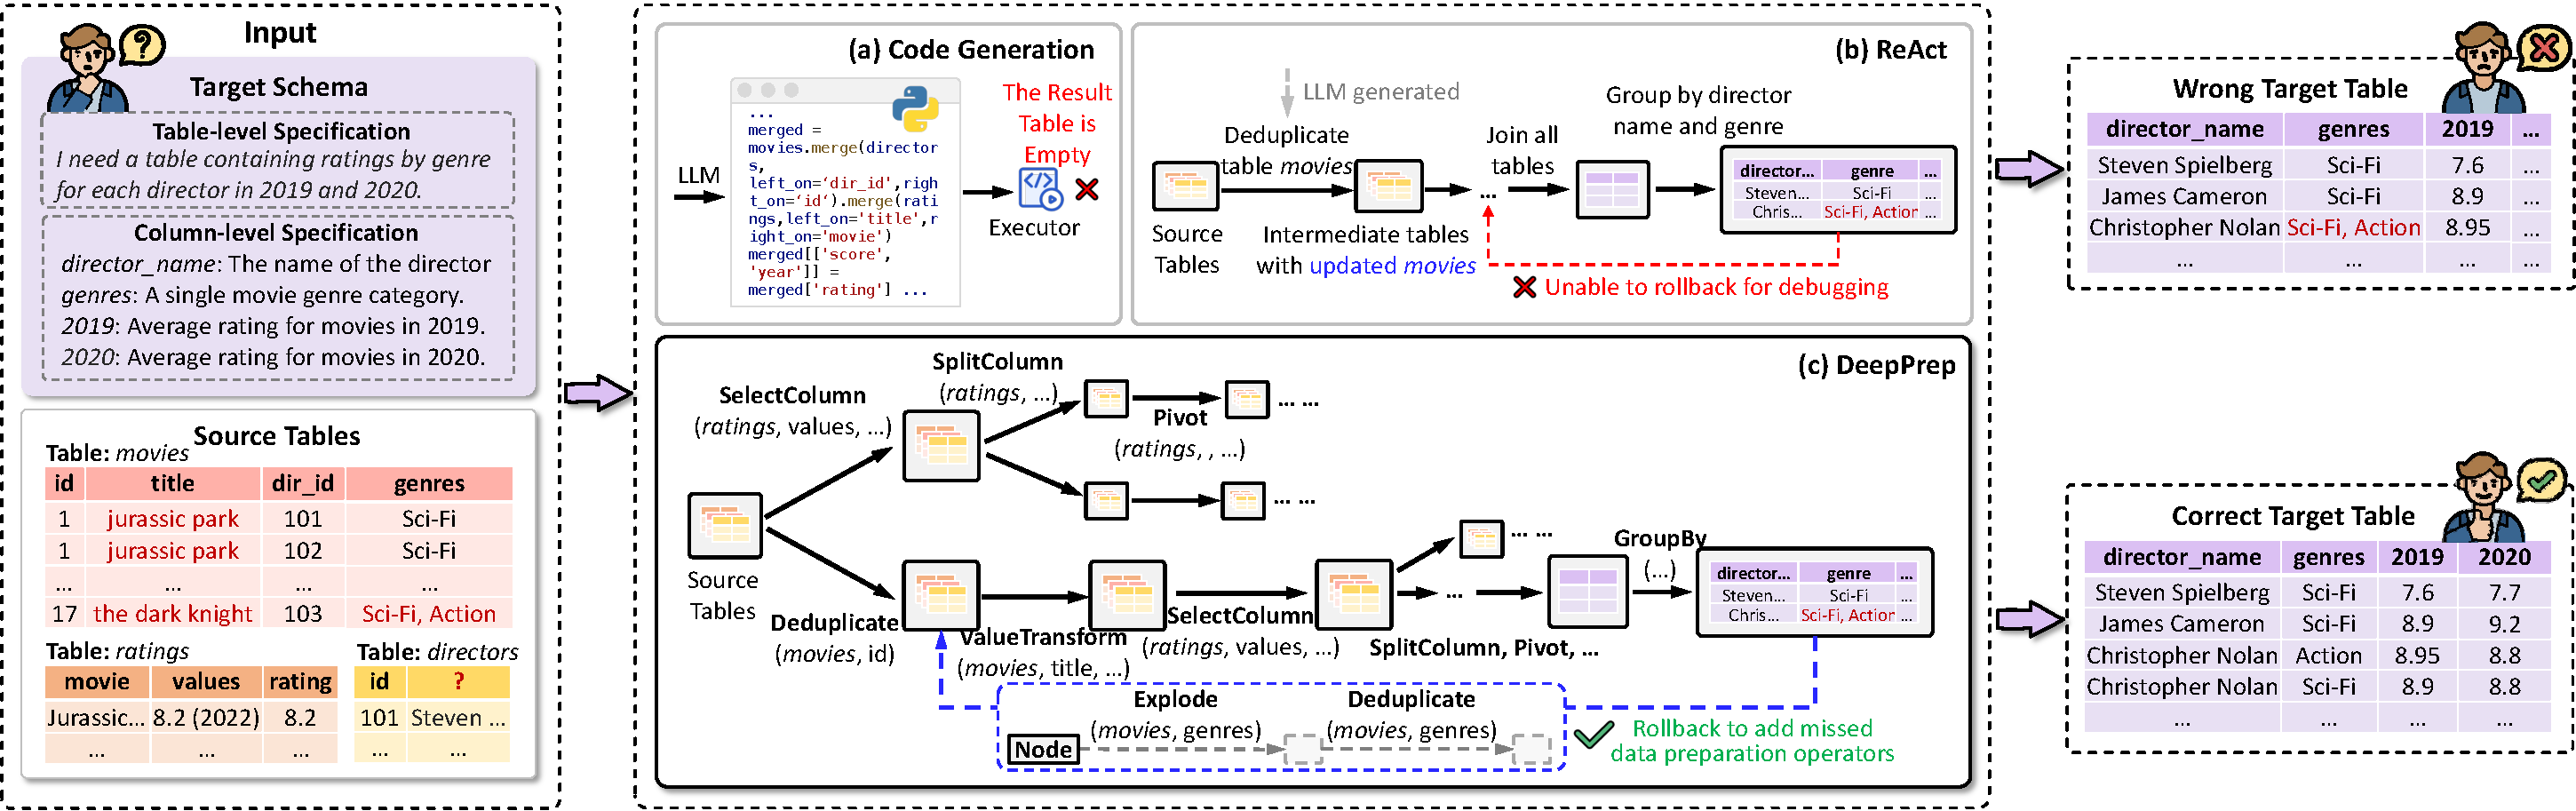
\includegraphics[width=0.95\textwidth]{figures/fig/introduction_example.pdf}
    \vspace{-1em}
    \caption{An illustrative example highlighting the core idea of \sys.
(a) Code generation makes decisions without grounding in intermediate execution results.
(b) ReAct-style approaches follow linear reasoning with limited ability to revise earlier decisions.
(c) \sys applies a tree-based structured exploration, which enables backtracking to resolve non-local errors.
    }
    \label{fig:introduction_example}
    \vspace{-1em}
\end{figure*}

Data preparation remains a major bottleneck in data science, often consuming 60\%--80\% of end-to-end analysis time~\cite{dasu2003exploratory}. 
This is due to the heterogeneity, noise, and misalignment across sources, as well as the iterative and interdependent nature of data preparation operations such as cleaning, joining, and aggregation.
% This is because real-world tables are heterogeneous, noisy, and misaligned across sources, and required transformations, such as cleaning, joining, and aggregation, are typically iterative and interdependent. 
To address these challenges, autonomous data preparation (ADP) aims to automatically transform multiple source tables into analysis-ready data based on a high-level target specification, by generating an executable transformation pipeline. For example, as shown in Figure~\ref{fig:introduction_experiment}, given several source tables and a target description such as ``\emph{I need a table containing \ldots}'', the system automatically generates and executes the required transformation steps.

%Data preparation (DP), the process of transforming raw tabular data into analysis-ready tables, remains a recurring bottleneck in data science. Prior studies estimate that DP can consume 60\%--80\% of end-to-end analysis time~\cite{dasu2003exploratory}, because real-world tables are heterogeneous, noisy, and misaligned across sources, and the required transformations are often tedious and iterative.
%
%This paper studies \textbf{Autonomous Data Preparation} (ADP). In ADP, the system takes multiple source tables $\mathcal{S}$ and a specification of the target schema $\Sigma^\ast$ as input, and {synthesizes a data-prep operator pipeline}, \ie a sequence of data preparation operations such as cleaning, reshaping, joining, and aggregation. The pipeline transforms $\mathcal{S}$ into an output table $\hat{T}$ matching $\Sigma^\ast$. As illustrated in Figure~\ref{fig:introduction_experiment}, an ADP system should accept heterogeneous source tables and a high-level target schema description (\eg ``The table contains \ldots''), then autonomously produce an executable transformation process that yields an analysis-ready table for downstream analytics.

\stitle{State-of-the-Art Approaches.}
Existing approaches to autonomous data preparation broadly fall into two categories.
%
\begin{itemize}[leftmargin=*]
    \item Traditional methods rely on rigid specifications such as input–output examples, transformation templates, or rule-based program synthesis~\cite{barowy2015flashrelate, singh2016blinkfill, he2018transform, jin2017foofah, huang2018auto}. While effective in constrained settings, these approaches are not designed to flexibly accommodate data preparation intent expressed in natural language.

%However, existing methods fail to realize this vision. Traditional approaches~\cite{barowy2015flashrelate, singh2016blinkfill, he2018transform, gulwani2012spreadsheet, jin2017foofah, heer2015predictive} rely on rigid specifications such as input-output examples of the target table or deterministic templates. They cannot robustly capture ambiguous, high-level analytical intent.

% Recent approaches leverage large language models (LLMs) to automate data preparation from natural language descriptions.
% A straightforward strategy prompts an LLM to generate a transformation pipeline in one shot, but such generation is often \emph{not execution-aware}: decisions are made without grounding in intermediate execution results, making runtime issues difficult to anticipate and resulting in brittle pipelines.
% Agentic approaches (\eg ReAct-style) partially mitigate this by interleaving reasoning with tool actions and incorporating execution feedback into subsequent decisions~\cite{yao2023react, aksitov2023rest}.
% However, most existing agentic pipelines follow a \emph{linear, append-only} interaction trajectory: earlier steps are not explicitly revisable, and recovery from non-local errors is difficult.
% In ADP, operator choices are strongly interdependent, and an early suboptimal decision (\eg premature join/aggregation or an irreversible reshape) may only manifest as a schema violation several steps later, where fixing the root cause requires rolling back and re-planning from an earlier state rather than patching locally.


\item Recent approaches leverage large language models (LLMs) to automate data preparation from natural language specifications~\cite{dong2024large,ruan2024language,lu2025large, zhang2026coda, deng2026taco}. Prompting-based methods generate data preparation code directly from task descriptions and examples~\cite{li2024towards, sapkota2025vibe, li2025weak}, but make decisions without systematic grounding in intermediate execution results, often leading to error-prone pipelines.
ReAct-style approaches incorporate execution feedback by interleaving reasoning with task-specific actions~\cite{yao2023react, aksitov2023rest}. However, this interaction follows a linear trajectory without explicit support for revising earlier decisions, which may be inadequate for autonomous data preparation, where early mistakes often become evident only after several dependent operations.
\end{itemize}

\stitle{Our Proposal.}
To address these limitations, we propose \textbf{\sys}, an LLM-powered agentic system for autonomous data preparation. \sys constructs data preparation pipelines through iterative, execution-grounded interaction with an environment that materializes intermediate table states and returns runtime feedback. 
Unlike one-shot code generation and linear ReAct-style interaction,
% which can only apply local fixes along a single trajectory, 
\sys organizes pipeline construction with \emph{tree-based agentic reasoning}.
This design enables structured exploration and \emph{non-local} revision when execution feedback indicates that earlier decisions are suboptimal.
Specifically, given source tables and a target schema, \sys operates in an iterative loop as below:
\begin{itemize}[leftmargin=*]
\item \textbf{Planning:} observing the current execution state and synthesizing a high-level plan for transforming existing tables.
% toward the target schema.
\item \textbf{Orchestration:} instantiating the plan as an executable operator pipeline with specified parameters.
\item \textbf{Execution:} executing the pipeline to materialize new table states and returning runtime feedback for subsequent decisions.
\end{itemize}
%
Through iterative interaction with execution feedback, \sys incrementally refines its decisions and converges to a data preparation pipeline that produces a table conforming to the target schema.
%
\begin{example}
\label{exam:intro_tree_advantage}
Consider the example in Figure~\ref{fig:introduction_example}. The goal is to construct a table for analyzing director performance across genres using audience ratings. A linear agent following a ReAct-style interaction may prematurely join and aggregate the data, resulting in multi-valued entries such as ``Sci-Fi, Action'' in the \textit{genre} column, which violates the target schema constraint requiring single-valued categories. Correcting this error requires revisiting an earlier cleaning decision on the \textit{movies} table, \ie inserting an \texttt{Explode} operation before reapplying downstream joins and aggregations.

\sys supports this naturally. 
% Instead of restarting the entire process,
It can backtrack to the execution state where the incorrect decision was made, expand an alternative branch with the corrected operation, and reuse valid operator prefixes from existing partial pipelines to produce a correct result.
% \fanj{Refine the example.}
\end{example}

%Beyond algorithmic limits, LLM-based ADP methods rely on \emph{closed-source} foundation models accessed via APIs, creating key deployment constraints:
%\textbf{(L1)} hidden architectures and training/inference details impede continuous, application-specific improvement; \textbf{(L2)} API-based access raises data privacy concerns because source tables and intermediate results must be sent to third-party providers; \textbf{(L3)} large LLMs incur substantial inference overhead and high monetary cost, making long-horizon, execution-grounded agentic interaction expensive.

% Recent approaches leverage large language models (LLMs) to automate data preparation from natural language descriptions, enabled by advances in natural language understanding and program generation. A straightforward strategy is to prompt an LLM with a task description and a few examples to generate a transformation pipeline~\cite{xxx}. However, such one-shot generation is not execution-aware, as decisions are made without grounding in intermediate execution results, making runtime issues difficult to anticipate and resulting in error-prone pipelines.
% ReAct-style approaches address this limitation by interleaving reasoning with task-specific actions and incorporating execution feedback into subsequent decisions~\cite{yao2023react, aksitov2023rest}. Nevertheless, this interaction follows a linear and append-only trajectory without explicit support for revising earlier steps. In ADP tasks, operator decisions are often interdependent, so early mistakes may appear only after several later steps and are difficult to correct under a linear interaction process.


%\stitle{LLM-powered Methods.}
%Large Language Models (LLMs) bring an opportunity to ADP due to strong natural language understanding and code synthesis capabilities.
%However, current LLM-powered baselines still exhibit two fundamental weaknesses.
%
%(1) {Direct prompting is not execution-aware.}
%A straightforward baseline is to directly prompt an LLM to generate a transformation script (\eg Python code or operator pipeline).
%Because this generation is decoupled from actual execution, it is prone to {schema hallucination}, where the model invents non-existent columns, mismatches data types, or assumes unavailable keys.
%These errors typically surface only at runtime, and without systematic execution feedback, the model has limited ability to self-correct.
%
%(2) {Agentic reasoning is execution-aware, but is brittle under linear search.}
%Agentic reasoning introduces an interactive loop where an LLM agent proposes an action, observes execution feedback, and revises subsequent actions.
%This execution-aware property can mitigate schema hallucination by grounding decisions in intermediate tables.
%Nevertheless, the dominant agentic baseline follows ReAct-style linear reasoning~\cite{yao2023react, aksitov2023rest}, which is inherently append-only and commits to a single trajectory.
%In ADP, operators have strong inter-dependencies, and early suboptimal decisions may only manifest as failures several steps later, making recovery require non-local revision rather than local patching.
%As a result, linear agentic baselines often fail on complex tasks that require explicit backtracking and structured exploration.


%\stitle{\sys: Tree-based Agentic Reasoning for ADP.}\
%To address these limitations, we propose \textbf{\sys}, an LLM-powered agentic system for ADP.
%\sys {constructs solutions explicitly as executable pipelines of predefined data-prep operators}, and organizes the search for such pipelines with {tree-based} agentic reasoning and a complementary training framework. The key idea is to represent pipeline construction as an {agentic reasoning tree}, where nodes materialize {environment states} (\ie sets of intermediate tables) and edges correspond to executed {operator instances}. This representation preserves alternative branches and enables {precise backtracking} to any prior state.
% The key idea is to

\stitle{Challenges and Solutions.}
We study the research challenges posed by the above agentic framework and outline our solutions.

The first challenge is how to support structured exploration and non-local backtracking under execution feedback.
To address this, \sys maintains an explicit tree of materialized execution states during pipeline construction, where nodes represent intermediate tables produced by executed operators and edges record the applied operator pipelines.
This representation enables execution feedback to be precisely attributed to earlier decision points, allowing the agent to backtrack and revise upstream choices when downstream failures occur.
Building on this structure, \sys introduces action-structured LLM interactions that operate directly over the tree, enabling the agent to incrementally expand, revise, or backtrack branches based on execution feedback.

The second challenge is how to effectively train LLMs for the tree-based agentic reasoning.
A straightforward solution is to apply reinforcement learning with outcome-level rewards~\cite{guo2025deepseek,le2022coderl}.
However, this setting introduces two difficulties.
First, \emph{reward sparsity}: long and interdependent pipelines make outcome insufficient for learning structured exploration and non-local backtracking.
Second, \emph{data scarcity}: existing ADP datasets focus on simple, short pipelines~\cite{DBLP:journals/pvldb/LiHYWC23, lai2025auto}, limiting supervision for multi-step, execution-aware reasoning.
To address these challenges, we propose a Progressive Agentic Training framework that (i) initializes the model with basic operator usage and tree-based interaction patterns, (ii) refines the policy through multi-turn reinforcement learning with a hybrid reward that considers both outcome-level and process-level signals, and (iii) leverages data synthesis to construct diverse and complex ADP tasks for training.

% \revise{
% \stitle{Differences from existing agentic solutions.} 
% % While \sys incorporates components common in recent agentic systems, its technical contribution lies in its specialized design for autonomous data preparation.
% \sys differs from existing systems in two key aspects. First, \sys performs tree-based agentic reasoning over explicit, materialized execution states. 
% Unlike ReAct~\cite{yao2023react}, which follows a linear trajectory, \sys can roll back to previously valid states and revise upstream decisions. 
% Unlike Tree-of-Thoughts~\cite{yao2023tree} and MCTS methods~\cite{li2025alphasql}, its search is grounded in executable data preparation operators and runtime feedback, and the resulting reasoning tree can be serialized into prompts for the subsequent reasoning.
% % over both successful and failed trajectories.
% %
% % Second, \sys proposes \textbf{Progressive Agentic Training}. Existing agentic systems are primarily designed for inference-time exploration and are not explicitly trained to follow a structured reasoning protocol. In contrast, \sys trains the model to execute tree-based agentic reasoning through control-tag supervision, execution-aware optimization, and a hybrid reward mechanism that combines outcome, partial, and process rewards.
% Second, \sys introduces progressive agentic training tailored to tree-based agentic reasoning in ADP. Specifically, our training method enables the model to gradually transition from learning the basic operator syntax to complex tree search, which cannot be addressed by existing agentic systems~\cite{zheng2025deepresearcher, jin2025search}. Moreover, we are the first to propose a verification-in-the-loop method for constructing diverse and complex ADP tasks for training.
% }

\stitle{Contributions.}
We summarize our contributions as follows.

\noindent
(1) We study the problem of autonomous data preparation with support for a wide range of data preparation operators (Section~\ref{sec:preliminary}), and introduce an LLM-powered agentic framework (Section~\ref{sec:overview}).

\noindent
(2) We propose two techniques to tackle the challenges of this problem: tree-based agentic reasoning for inference (Section~\ref{sec:tree_based_agentic_reasoning}) and progressive agentic training for agent optimization (Section~\ref{sec:agentic_training_framework}).

\noindent
(3) We conduct extensive experiments on real-world ADP benchmarks.
Results show that \sys achieves accuracy comparable to closed-source models (\eg GPT-5) at {15$\times$} lower inference cost, while establishing state-of-the-art performance among open-source baselines and generalizing well across diverse datasets.

\noindent
(4) We release the code, data, and a comprehensive set of trained model weights (from 0.5B to 14B parameters), enabling users to deploy ADP agents under different computational budgets.
% \footnote{Accessible via: https://anonymous.4open.science/r/DeepPrep-0432}.
% at Github\footnote{\url{https://github.com/ruc-datalab/DeepPrep}} and Huggingface\footnote{\url{https://huggingface.co/RUC-DataLab/DeepPrep}}


% \fanj{xxx} (Section~\ref{sec:experiment}).